\documentclass[aps,prl,twocolumn,showpacs]{revtex4}
\usepackage{graphicx}
\usepackage{epstopdf}
%\usepackage{float}

\begin{document}

\title{A successful solar model using new solar composition data}

\author{
\mbox{Sunny Vagnozzi{$^{1,2}$},}
\mbox{Katherine Freese{$^{1,3}$},}
and
\mbox{Thomas H. Zurbuchen{$^{4}$}}
}

\affiliation{
\mbox{$^1$ The Oskar Klein Centre for Cosmoparticle Physics, Stockholm University, SE-106 91 Stockholm, Sweden}
\mbox{$^2$ NORDITA, KTH Royal Institute of Technology and Stockholm University, SE-106 91 Stockholm, Sweden}
\mbox{$^3$ Michigan Center for Theoretical Physics, Department of Physics, University of Michigan, Ann Arbor, MI 48109, USA} 
\mbox{$^4$ Department of Climate and Space Sciences and Engineering, University of Michigan, Ann Arbor, MI 48109, USA}
\\
{\tt sunny.vagnozzi@fysik.su.se},
{\tt ktfreese@umich.edu},
{\tt thomasz@umich.edu}
}

\begin{abstract} \noindent

A resolution is proposed to the ``solar abundance problem", that is, the discrepancy between helioseismological observations and the predictions of solar models, computed implementing state-of-the-art photospheric abundances. We reassess the problem considering a newly determined set of abundances, which indicate a lower limit to the metallicity of $Z_{\odot} = 0.0196 \pm 0.0014$, significantly higher than findings during the past decade. Such value for the metallicity is determined in situ, measuring the least fractionated solar winds over the poles of the Sun, rather than spectroscopically. We determine the response of helioseismological observables to the corresponding changes in elemental abundances. Our findings indicate that, taking inversion errors into account, good agreement between models and observations is achieved. The definitive test for these abundances will be measurements of the CNO neutrino fluxes by SNO$^+$ (which we expect to be $\sim$ 30-50\% higher than predictions using abundances based on photospheric spectroscopy). We briefly comment on the implausibility of previously proposed solutions based on dark matter. The results also imply that 3D spectroscopic inversion processes systematically underestimate elemental abundances in the photosphere. Our conclusion is that the solar abundance problem has found a definitive compelling solution.

\end{abstract}

\pacs{96.60.Fs., 96.60.Ly}

\maketitle

\textbf{\textit{Introduction.\/}}\---Among the most important diagnostics of the evolutionary history of the Sun is its metallicity $Z_{\odot}$, defined as the fraction of the solar mass residing in elements heavier than He. In the standard solar model (SSM), absolute and relative elemental abundances are treated as inputs, from which observables to be compared with helioseismological inferences are obtained. Up to 1998, heavy element mixtures provided by Anders \& Grevesse (AG89, $Z_{\odot} = 0.0202$) \citep{ag89}, and subsequently by Grevesse \& Sauval (GS98, $Z_{\odot} = 0.0170$) \cite{gs98} yielded acceptable concordance between model and data. In recent years, however, an important dilemma known as the ``solar abundance problem" has emerged. A systematic reassessment of solar model atmospheres has led to a downward revision of the photospheric abundances of heavy elements (e.g. \cite{ala01,agsa04,caffau,agss15i,agss15ii,agss15iii}). Particularly noteworthy are the revisions known as AGS05 \cite{ags05} and AGSS09 \cite{agss09}, which yield $Z_{\odot} = 0.0122$ and $0.0133$ respectively. These revisions rely on novel 3D inversion models for the inversion of spectroscopic data to photospheric abundances replacing the previous status quo of 1D or 2D models. \newline \indent
%
The effect of such revisions has been that of spoiling the otherwise good agreement between solar models and results from helioseismology \cite{disagreement1,bahcallserenelli1,bahcallserenelli3,disagreement2,penagaray,serenellibasu,bergemann}. For instance, the sound speed $u(r)$ is inferred to be $\sim 1\%$ lower than predicted at the bottom of the convective envelope (amounting to a discrepancy of $\sim 10\sigma$). Similarly, the surface He abundance $Y_s$ and convective zone boundary (CZB) $R_b$ are $\sim 7\%$ lower and $\sim 1.5\%$ higher than those deduced from helioseismology, corresponding to $\sim 6\sigma$ and $\sim 15\sigma$ discrepancies respectively \cite{villante4}. %Moreover, analyses of low-degree acoustic oscillations by the BiSON network \cite{bison} indicate that these disparities cannot be ascribed to incorrect modeling of the solar convective zone \cite{elsworth1,elsworth2}.
Various solutions to the problem have been proposed, ranging from an anomalously large Ne abundance in the photosphere \cite{bahcallneon}, physical processes not accounted for in the SSM (e.g. \cite{lowz1,lowz2,lowz3,mass,effects,solution2,solution3,enhanced1,solution1,yang2016}), incorrectly estimated opacity \cite{solution4,gazit}, to axion-like particles \cite{lightbosons} and exotic energy transport due to captured dark matter (DM) \cite{frandsen,silk,bertone,panci,psq2,psq2long,dev}. However, none of these solutions appears compelling (e.g. \cite{shearer2014}). It is resolving the discrepancies in the three observables $Y_s, R_b,$ and $u(r)$ that we shall focus on in our work. \newline \indent
%
In this Letter, we investigate a simple solution to the SSM problems, our assertion being that novel photospheric abundances have been incorrectly inferred. This approach is motivated by a completely different methodology to estimate photospheric abundances, based on \textit{in situ} measurements of heavy ions in the least fractionated solar wind. Adopting the latest set of abundances thus determined, we assess the effect of the new elemental abundances on helioseismological observables. We do so by using the \textit{Linear solar model} formalism \cite{villante5}, which allows us to determine the response of the Sun to arbitrary modifications of input parameters. Using this methodology we explore the consistency of these new abundance measurements with constraints from helioseismology. \newline \indent
%
\textbf{\textit{In situ metallicity determination.\/}}\---We here compare new \textit{in situ} estimates of the solar metallicity with those that rely on photospheric spectroscopy. The latter technique has found broad use within the community.  Yet the interpretation of observations using photospheric spectroscopy is anything but straightforward.  It requires sophisticated inversion techniques that take into the account radiative transport, three-dimensional structure and hydrodynamic models of the observation volumes, along with departures from local thermal equilibrium. In addition, the methodology also relies on detailed knowledge of the relevant atomic and molecular transition probabilities \cite{agss09,caffau}. \newline \indent
%
Alternatively, metallicity can be inferred from \textit{in situ} collection of solar samples. Whereas these techniques do not suffer from the aforementioned technical difficulties, they are in general subject to different challenges, such as fractionation processes that tend to enrich or deplete ions based on their ionization and transport histories. Processes known to be at work are collisional coupling, especially for He, First Ionization Potential (FIP) fractionation processes presumably operating in the low solar atmosphere, and gravitational settling \cite{geiss,gravitational}. \newline \indent
%
However, it has been shown and recently confirmed that most if not all of these processes are either absent or significantly reduced in solar wind emerging from polar regions near solar minimum, out of polar coronal holes (PCHs) \cite{z6,z12}. The most significant residual fractionation effect in this wind is that of insufficient collisional coupling that affects all of solar wind, but is most evident in He/H \cite{geiss}. Furthermore, it was shown that the composition of these PCHs is constant during the entire \textit{Ulysses} mission \cite{ulysses}, which explored these regions during its mission from 1990 to 2009. The only observed residual changes relate to small changes of the ionization state, reflecting the temperature and acceleration history of the solar wind emerging from PCHs. The elemental composition remains constant within the error bars of this methodology \cite{mc,z11}. \newline \indent
%
It follows that the sample collected from PCHs provides a direct measurement of the photospheric composition with one caveat:  \cite{z16} (which we will refer to as vSZ16 henceforth) cannot exclude a small residual fractionation in these regions. However, based on the physical processes and a systematic study of various source regions, they concluded that such processes systematically decrease the overall solar metallicity. The \textit{in situ} measured $Z_{\odot}$ value therefore constitutes a lower limit on the photospheric $Z_{\odot}$, allowing for a consistency check of the values determined via photospheric spectroscopy and also constraints from helioseismology. In our analysis we choose to restrict ourselves to the PCH abundances provided by vSZ16 because it has been conclusively shown to be most similar to the photosphere, in contrast to low-latitude solar wind which is more prone to fractionation \cite{feldman,reisenfeld,z16}. The data are provided by the \textit{Ulysses} mission, and particularly by its ``Solar Wind Ion Composition Spectrometer" (SWICS) \cite{swics}. \newline \indent
%
The derived metallicity is $Z_{\odot} = 0.0196 \pm 0.0014$, a figure which is significantly larger than those of the AGS05 \cite{ags05} and AGSS09 \cite{agss09} catalogues, and intermediate between the AG89 \cite{ag89} and GS98 \cite{gs98} ones. Although one might be tempted to jump to the hasty conclusion that this revised value automatically restores agreement between models and helioseismology, care must be taken. The details of such statement crucially depend on the exact variation of the abundances of individual metals in our Sun, since different metals affect the radiative opacity of the solar mixture (and thereby the response of helioseismological observables) in a different way. In other words, the total metallicity does not uniquely determine the response of the Sun because it is degenerate with the individual metal abundances (the same change in the total metallicity can be obtained by varying the abundances of distinct elements differently). \newline \indent
%
\textbf{\textit{Linear solar model.\/}}\---To investigate the impact of varying input parameters (such as individual elemental abundances) on helioseismological observables we need to be able to quantify the response of the Sun to arbitrary variations of these parameters. We exploit the recently developed \textit{Linear solar model} (LSM hereafter) approach \cite{villante5,villante4}. Herein, the solar structure equations are linearized, resulting in a set of ordinary differential equations for the fractional variations of the thermodynamic quantities describing the Sun. The LSM has been shown to reproduce the predictions of full nonlinear evolutionary codes to a high level of accuracy \cite{villante5}. \newline \indent
%
The effect of varying the metallicity of the Sun is to modify its radiative opacity profile, $\kappa (r)$. This, in turn, is a key quantity that describes the coupling between radiation and matter in the hot dense interior of the Sun. It plays a pivotal role in the determination of helioseismological observables. Leaving aside intrinsic opacity variations (that is, opacity variations with a fixed composition), the fractional opacity variation we will be concerned with is the \textit{composition} opacity variation $\delta \kappa _Z(r)$, driven by a change in elemental abundances. Thus we can express the fractional opacity variation as \cite{villante3}:
%
\begin{eqnarray}
\delta \kappa (r) \approx \delta \kappa _Z (r) \simeq \sum _j \frac{\partial \ln \kappa (r)}{\partial \ln Z_j}\delta Z_j \equiv \sum _j \kappa _{Z_j}\delta Z_j \, .
\label{deltakappaz}
\end{eqnarray}
%
In Eq.(\ref{deltakappaz}), the sum runs over the eight metals which contribute to $\sim 98\%$ of the Sun's metallicity: C, N, O, Ne, Mg, Si, S, and Fe. For each of these metals, $\delta Z_j$ represents the fractional change in abundance with respect a chosen baseline set of abundances (which we take to be those the AGSS09 catalogue). \newline \indent
%
\begin{figure}[t]
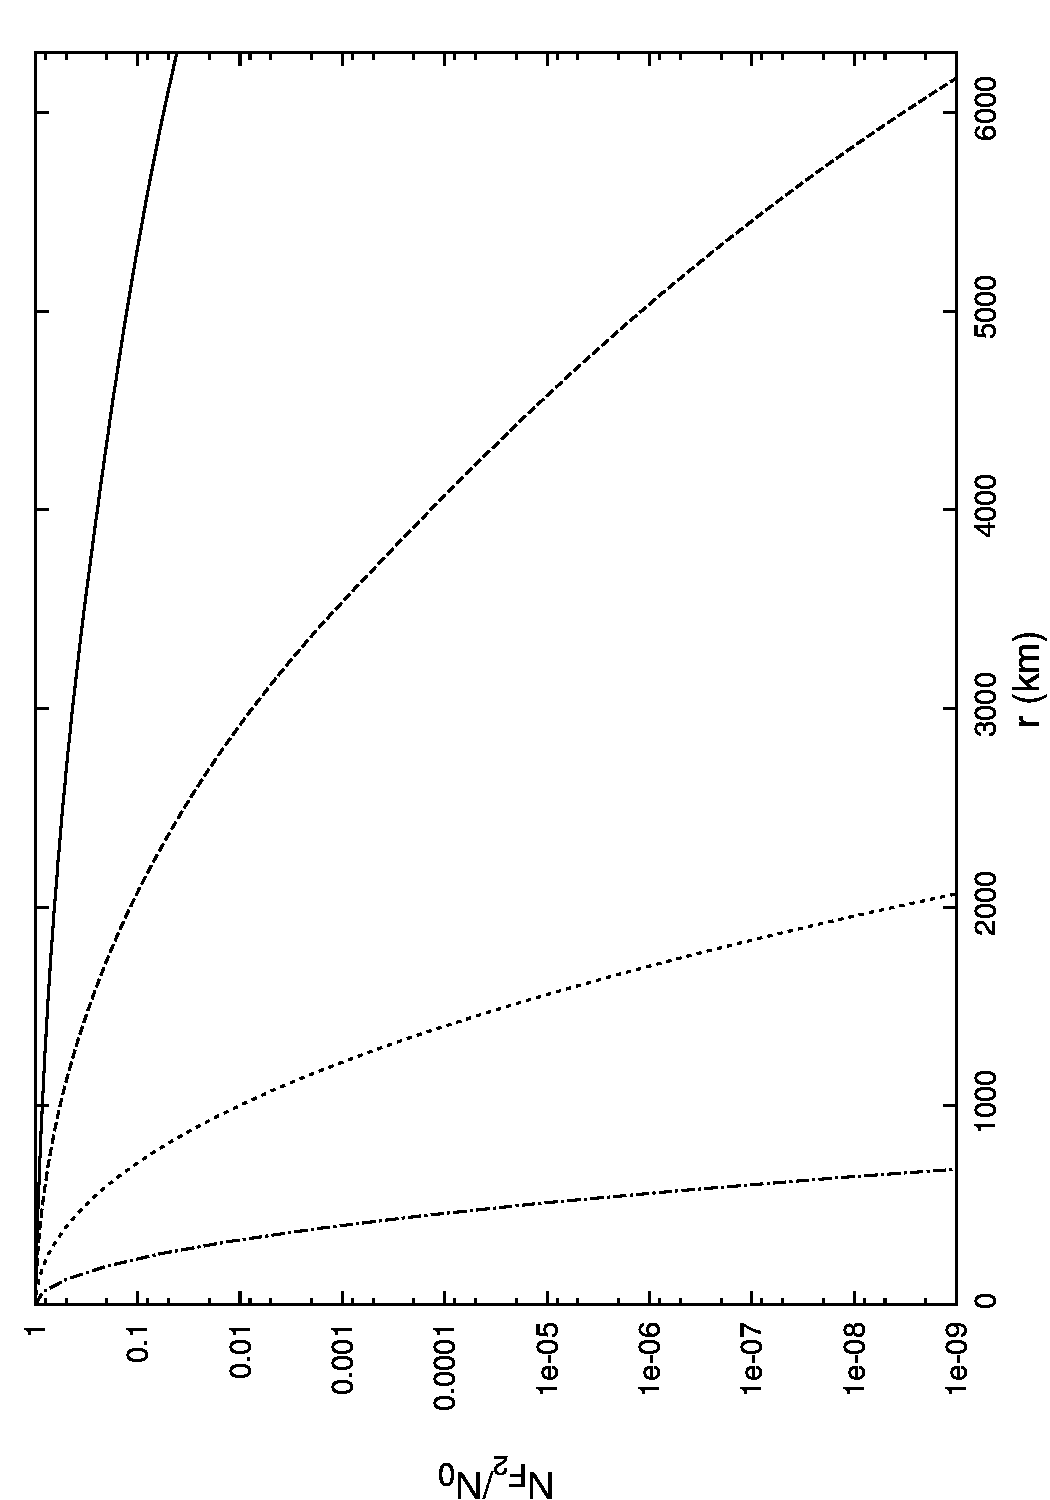
\includegraphics[width=.3\textwidth , angle=270]{fig1.eps}
%\vskip -0.4 cm
\caption{Logarithmic derivatives of opacity with respect to individual metal abundances.}
\label{fig1}
\end{figure}
\begin{table}[tb]
%\vskip -0.4 cm
\caption{Elemental abundances for the AGSS09 and vSZ16 catalogues, and fractional variation between the two. For all elements other than Ne, the new element abundances obtained from \textit{in situ} vSZ16 measurements are significantly higher.}
\label{tab1}
\begin{tabular}{c c c c}
\hline\hline \vspace{-4mm}\\
 \ \ \ Element \ \ \ & \ \ \ $\epsilon_{_{\text{AGSS09}}}$ \ \ \ & $\epsilon_{_{\text{vSZ16}}}$ \ \ \ & \ \ \ $\delta Z_i$ \ \ \ \\      
\hline
 \ \ \ C \ \ \ & \ \ \ $8.43 \pm 0.05$ \ \ \ & \ \ \ $8.65 \pm 0.08$ \ \ \ & \ \ \ $0.66 \pm 0.15$ \ \ \ \\
 \ \ \ N  \ \ \ & \ \ \ $7.83 \pm 0.05$ \ \ \ & \ \ \ $8.97 \pm 0.08$ \ \ \ & \ \ \ $0.38 \pm 0.08$ \ \ \ \\
 \ \ \ O \ \ \ & \ \ \ $8.76 \pm 0.07$ \ \ \ & \ \ \ $8.82 \pm 0.11$ \ \ \ & \ \ \ $0.35 \pm 0.10$ \ \ \ \\
 \ \ \ Ne \ \ \ & \ \ \ $7.93 \pm 0.10$ \ \ \ & \ \ \ $7.79 \pm 0.08$ \ \ \ & \ \ \ $-0.28 \pm 0.08$ \ \ \ \\
 \ \ \ Mg \ \ \ & \ \ \ $7.60 \pm 0.04$ \ \ \ & \ \ \ $7.85 \pm 0.08$ \ \ \ & \ \ \ $0.78 \pm 0.16$ \ \ \ \\
 \ \ \ Si \ \ \ & \ \ \ $7.51 \pm 0.03$ \ \ \ & \ \ \ $7.82 \pm 0.08$ \ \ \ & \ \ \ $1.04 \pm 0.21$ \ \ \ \\
 \ \ \ S \ \ \ & \ \ \ $7.12 \pm 0.03$ \ \ \ & \ \ \ $7.56 \pm 0.08$ \ \ \ & \ \ \ $1.75 \pm 0.35$ \ \ \ \\
 \ \ \ Fe \ \ \ & \ \ \ $7.50 \pm 0.04$ \ \ \ & \ \ \ $7.73 \pm 0.08$ \ \ \ & \ \ \ $0.70 \pm 0.15$ \ \ \ \\
\hline
\end{tabular}
\end{table}
The logarithmic derivatives $\kappa _{Z_j}$ are given in \cite{villante3}, and plotted in Figure \ref{fig1}. In Table \ref{tab1} we list the elemental abundances $\epsilon _i$ of these eight metals in the AGSS09 and vSZ16 catalogues. The fractional variation in abundance for a given element $i$ is determined as:
%
\begin{eqnarray}
\delta Z_i = 10^{(\epsilon_{_{\text{AGSS09}},i}-\epsilon_{_{\text{vSZ16}},i})}-1
\end{eqnarray}
%
For all elements other than Ne, the new element abundances obtained from \textit{in situ} vSZ16 measurements are significantly higher. In particular, for Si and S, the fractional increase is $\gtrsim$100\%. We note that \cite{shearer} estimate systematic errors at most $\sim 20\%$ for the vSZ16 catalogue. Through Eq.(\ref{deltakappaz}) we estimate the fractional variation in radiative opacity $\delta \kappa (r)$ due to the change in elemental abundances between the AGSS09 and vSZ16 catalogues. The results are presented in Figure \ref{fig2}.%\footnote{Recent works have determined that a smooth opacity variation from $\sim 10\%$ in the core to $\sim 30\%$ near the convective zone boundary can restore the agreement between models and helioseismology \cite{villante3,villante4}. However, due to various degeneracies, this is not the unique $\delta \kappa (r)$ which can solve the problem. Moreover, this $\delta \kappa (r)$ was determined with several simplifying assumptions which do not hold in our case, thus we are not concerned with the fact that our profile does not exactly reproduce the one found in \cite{villante3,villante4}. Nonetheless, model-independent considerations univocally determine the required opacity variation at the convective radius, $\delta \kappa _b \simeq 0.24 \pm 0.03$ \cite{villante4}. In Figure \ref{fig2} the corresponding 2$\sigma$ band is denoted by the tick around $r/R_{\odot} \simeq 0.73$. Thus, although our opacity profile does reproduce the one in \cite{villante3,villante4}, the model-independent relation for $\delta \kappa _b$ is satisfied within $\lesssim 2\sigma$.}.
\begin{figure}[!h]
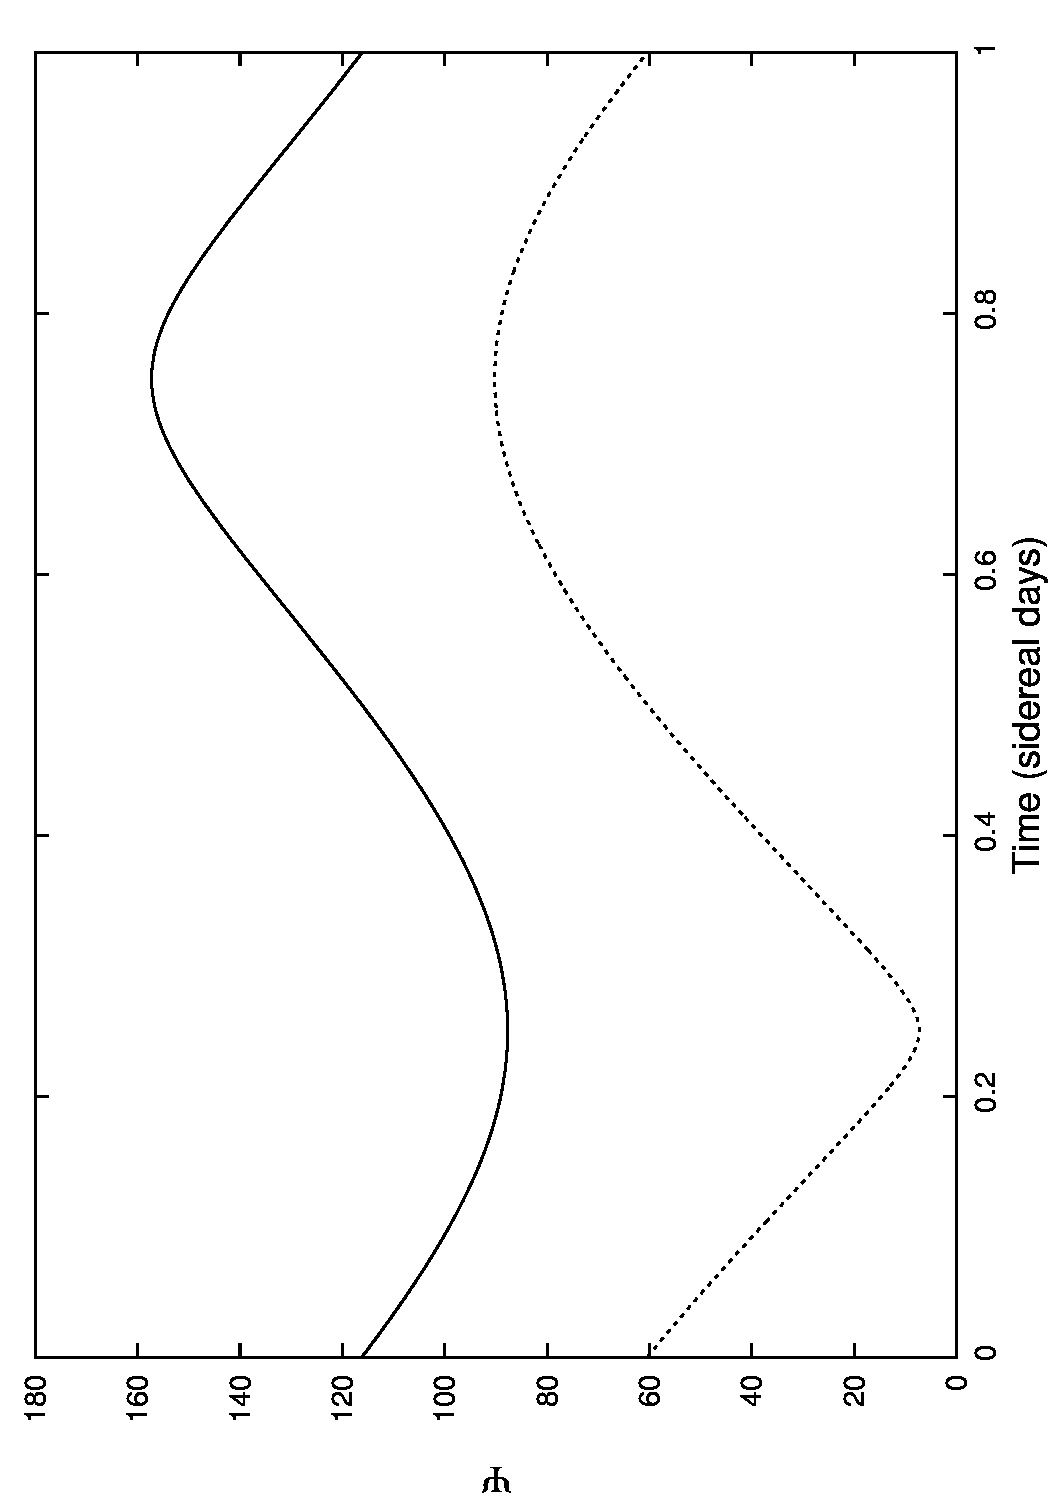
\includegraphics[width=.3\textwidth , angle=270]{fig2.eps}
%\vskip -0.4 cm
\caption{Fractional variation in opacity $\delta \kappa (r)$ when going from AGSS09 to vSZ16 abundances.}
\label{fig2}
\end{figure}

The fractional opacity variation, $\delta \kappa (r)$, allows us to estimate the response of helioseismological observables to variations in the metallicity content of the Sun. For $\delta \kappa (r) \lesssim 1$, the response of the Sun is linear. Thus the variation of a generic given quantity $\delta Q \equiv Q/\overline{Q}-1$ (where $\overline{Q}$ is the SSM value for $Q$) can be related to the opacity variation $\kappa (r)$ through a kernel $K_Q(r)$ as:
%
\begin{eqnarray}
\delta Q = \int dr \ K_Q(r)\delta \kappa (r) \, .
\label{kernel}
\end{eqnarray}
%
Here the kernel $K_Q(r)$ corresponds to the functional derivative of $Q$ with respect to the opacity, and quantifies the sensitivity of the given quantity to opacity variations in different zones of the Sun. \newline \indent
The kernels for surface He abundance and CZB, $K_Y(r)$ and $K_R(r)$, have been worked out in \cite{villante4} and are plotted in Figures \ref{fig3} and \ref{fig4}.%Notice that the kernel for the convective radius averages to zero (this is true also for the sound speed kernels, although we haven't shown them here), which means that these two observables are insensitive to a global rescaling of the opacity profile, but just to its tilt.
\begin{figure}[!h]
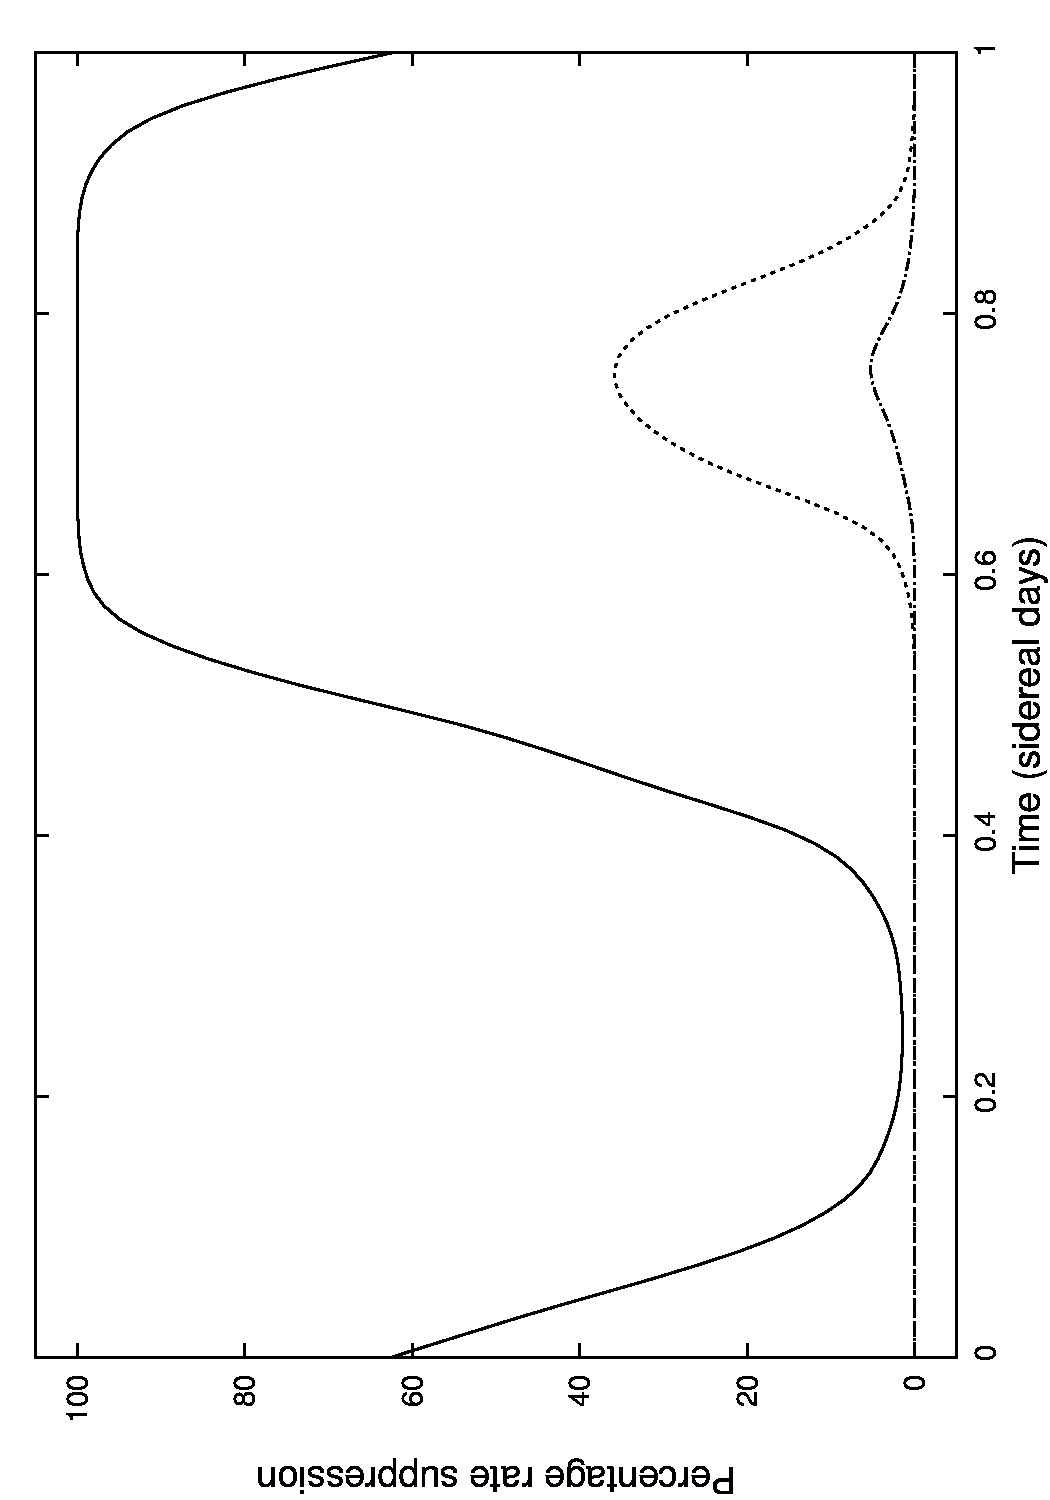
\includegraphics[width=.3\textwidth , angle=270]{fig3.eps}
%\vskip -0.4 cm
\caption{Functional derivative $K_Y(r)$ of surface He abundance with respect to opacity.}
\label{fig3}
\end{figure}
\begin{figure}[!h]
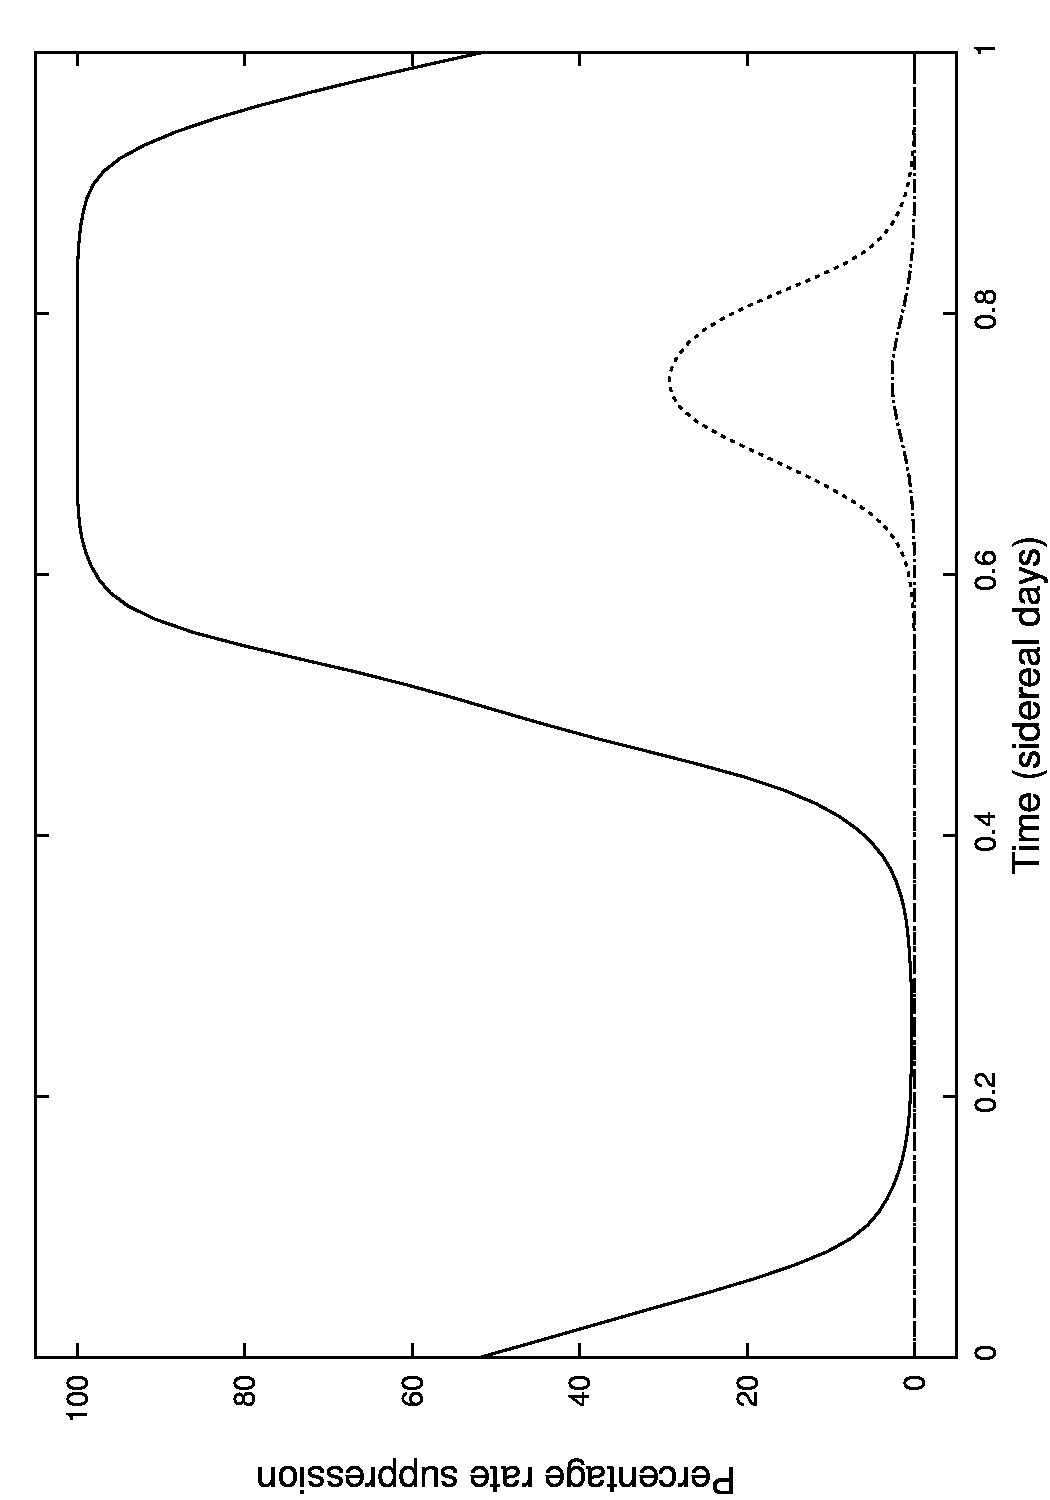
\includegraphics[width=.3\textwidth , angle=270]{fig4.eps}
%\vskip -0.4 cm
\caption{Same as Fig. \ref{fig3} for convective radius, $K_R(r)$.}
\label{fig4}
\end{figure}
The functional derivatives of the sound speed profile (at a given $r'$) with respect to opacity, $K_u(r,r')$, have also been worked out in \cite{villante4} for a few $r'$s. However, for our purposes it is more immediate to use the logarithmic derivatives of the sound speed with respect to the elemental abundances. These have been calculated in \cite{villante3} using the LSM formalism and are plotted in Figure \ref{fig5}. Similarly to the case with opacity in Eq.(\ref{deltakappaz}), we can then reconstruct the response of the sound speed profile according to:
%
\begin{eqnarray}
\delta u (r) \simeq \sum _j \frac{\partial \ln u(r)}{\partial \ln Z_j}\delta Z_j \equiv \sum _j u_{Z_j}\delta Z_j \, ,
\label{deltaur}
\end{eqnarray}
%
\begin{figure}[!h]
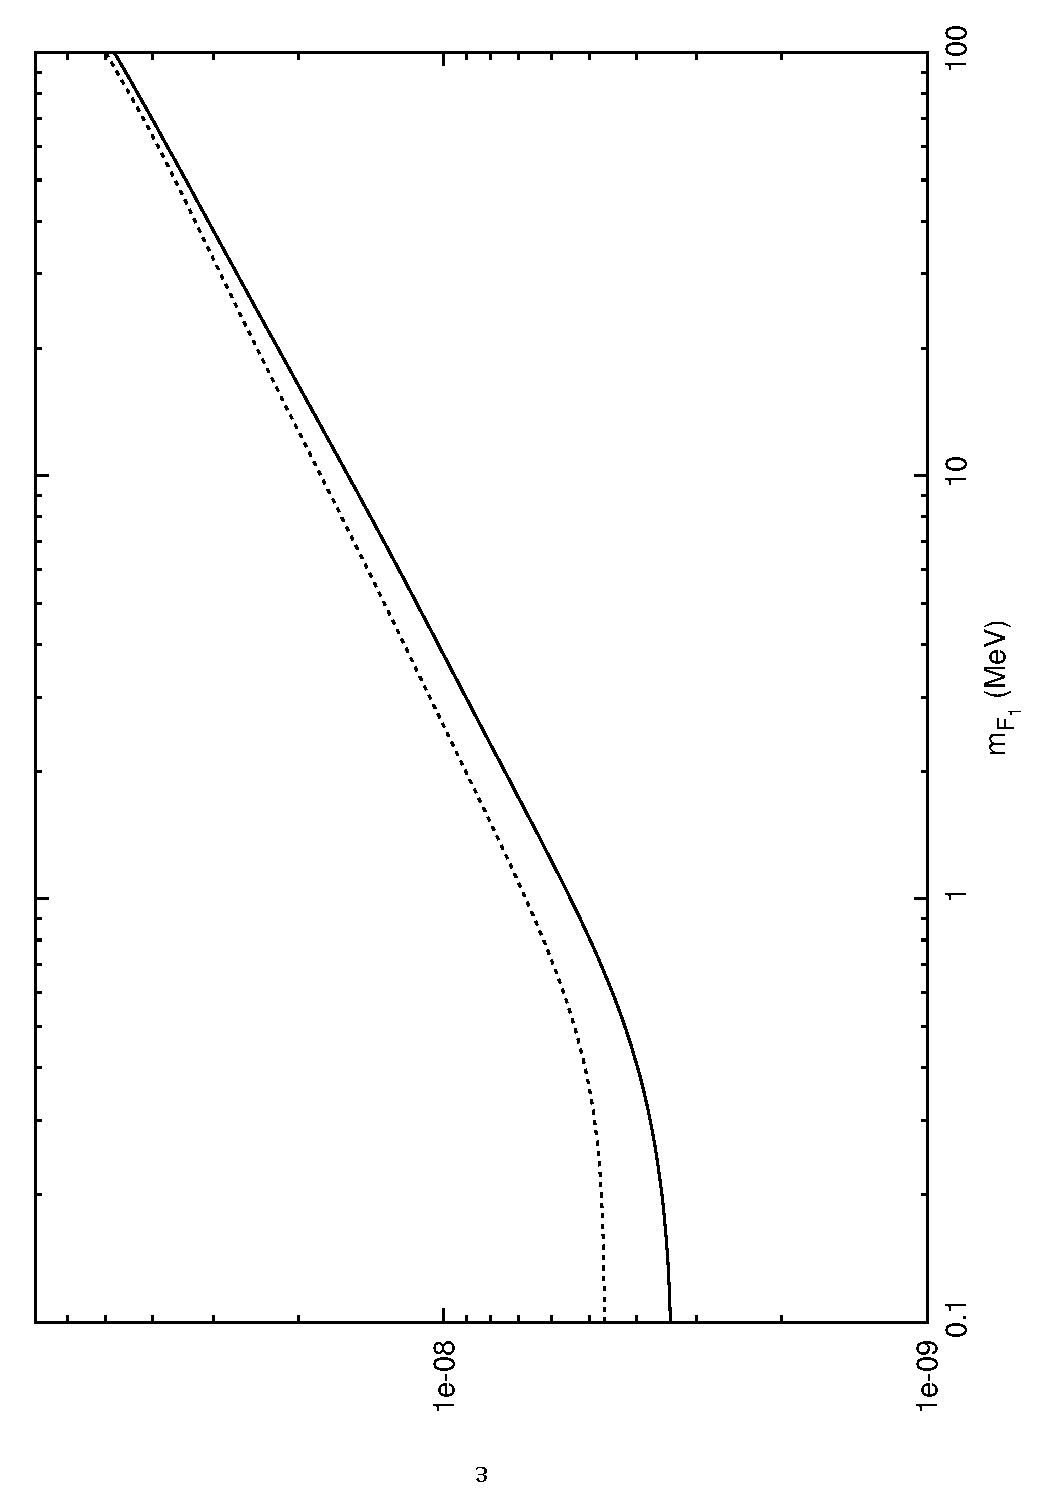
\includegraphics[width=.3\textwidth , angle=270]{fig5.eps}
%\vskip -0.4 cm
\caption{Logarithmic derivatives of sound speed with respect to individual metal abundances.}
\label{fig5}
\end{figure}

\textbf{\textit{Results.\/}}\---Using the previously discussed approach, we evaluate the response of the three helioseismological observables of interest: surface He abundance $Y_s$, CZB $R_b$, and sound speed $u(r)$ (particularly at the bottom of the convective envelope). We begin by considering the fractional sound speed variation $\delta u$, gauged using Eq.(\ref{deltaur}). The result is shown in Figure \ref{fig6}, where we also plot 1$\sigma$ and 2$\sigma$ error bands on $\delta u$, obtained by propagating the uncertainties on $\delta Z_j$. The obtained reponse $\delta u$ is to be compared with the thick solid line in the figure: this represents the fractional difference between the AGSS09 radial sound speed profile and the one inferred from helioseismology (see e.g. \cite{psq2}). It thus amounts to the fractional variation required to bring the AGSS09 sound speed in agreement with helioseismological inferences. Henceforward we will refer to this profile as $\delta u_{\text{th}}$.
\begin{figure}[!h]
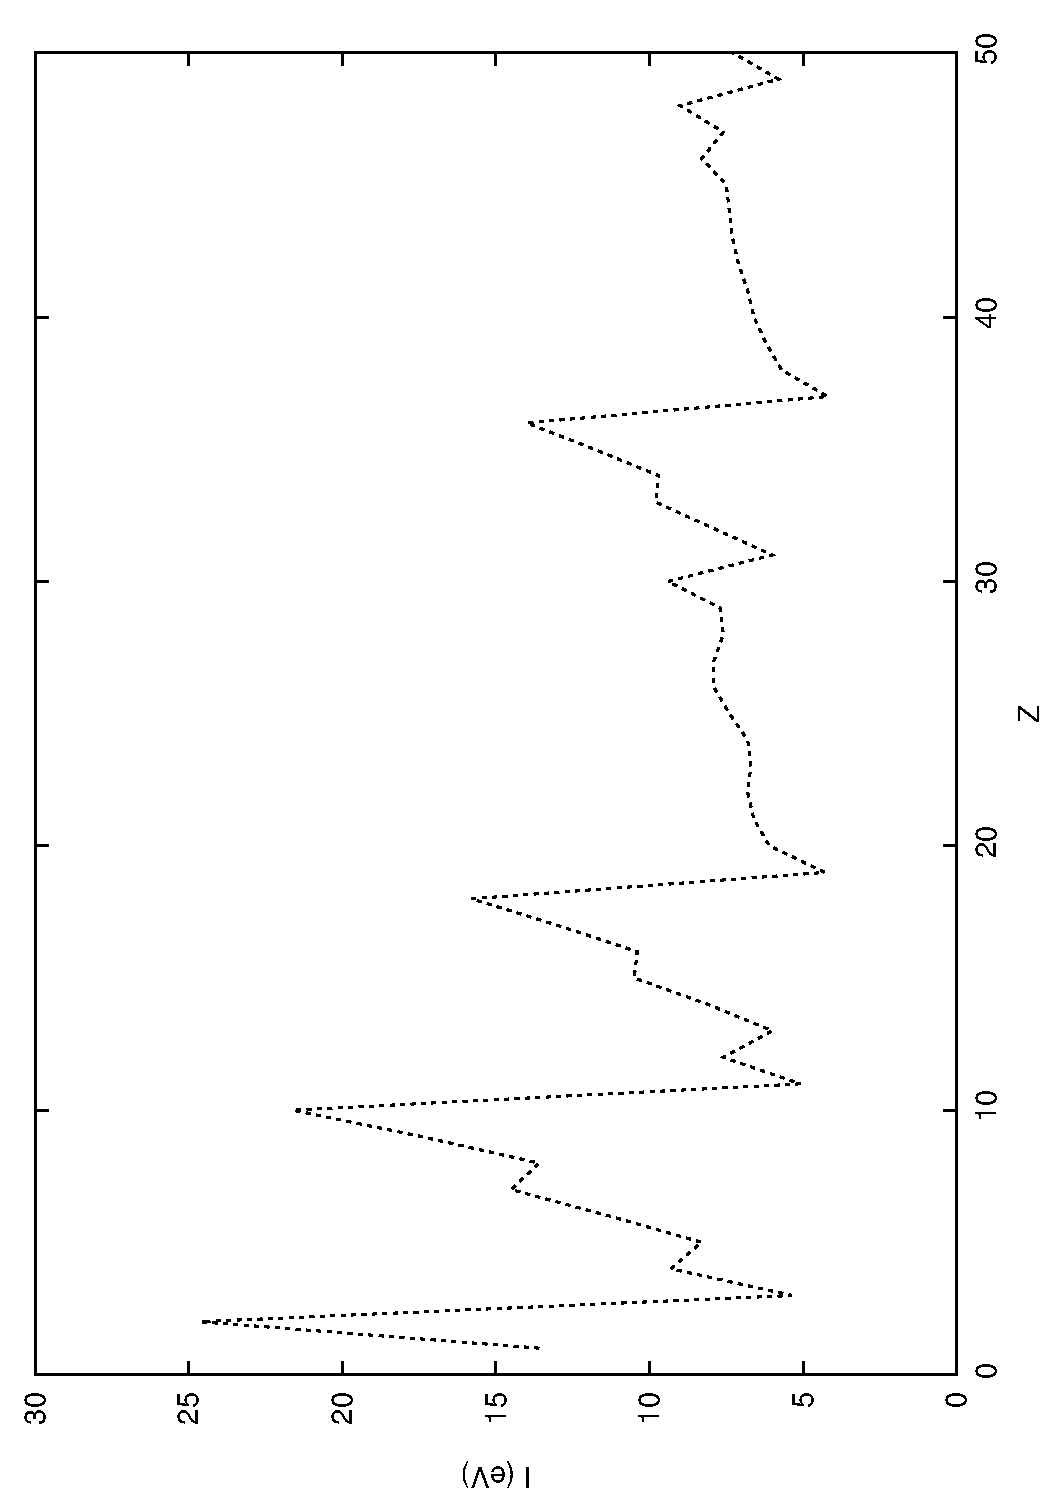
\includegraphics[width=.35\textwidth , angle=270]{fig6.eps}
%\vskip -0.4 cm
\caption{Response of sound speed when going from AGSS09 to vSZ16 abundances, with 1$\sigma$ and 2$\sigma$ bands. Thick solid line is $\delta u_{\text{th}}$ (variation which brings AGSS09 sound speed in agreement with helioseismology), with dashed and dotted-dashed lines representing 1$\sigma$ statistical and conservative helioseismological uncertanties. CZB boundary located at $r/R_{\odot} \simeq 0.73$.}
\label{fig6}
\end{figure}

To complete the analysis of the sound speed response $\delta u(r)$, we include uncertainties on $\delta u_{\text{th}}(r)$ (thick solid line in Figure \ref{fig6}). By far the largest source of uncertainty is the one coming from helioseismological inversion \cite{helioseismologyuncertainty1,helioseismologyuncertainty2,helioseismologyuncertainty3}, and \cite{helioseismologyuncertainty1} first discussed two different approaches to estimating such uncertainties. The first is the ``\textit{statistical}" approach, wherein it is assumed that different contributions to the total uncertainty partially compensate each other and are added in quadrature. This approach is most justified when the partial uncertainties essentially all correspond to statistical uncertainties in the measured frequencies of solar $p$-modes. A second approach, denoted as ``\textit{conservative}", adds up partial uncertainties linearly, and results in a total uncertainty which is larger than the statistical one by a factor of $\sim$2-3. This approach is best suited when one has reason to believe that the main helioseismological uncertainties are of systematic nature, e.g. related to residual model-dependence (treatment of opacities, equation of state, diffusion) and/or inversion method. The authors of \cite{helioseismologyuncertainty1} argue that the conservative approach actually provides the best estimate of the uncertainty. For $r/R_{\odot} \lesssim 0.1$ the helioseismology uncertainty is quite large, reflecting the fact that the reconstructed sound speed in this region is highly uncertain due to the low number of low-$l$ $p$ modes reaching the most inner regions our Sun.
\begin{figure}[!h]
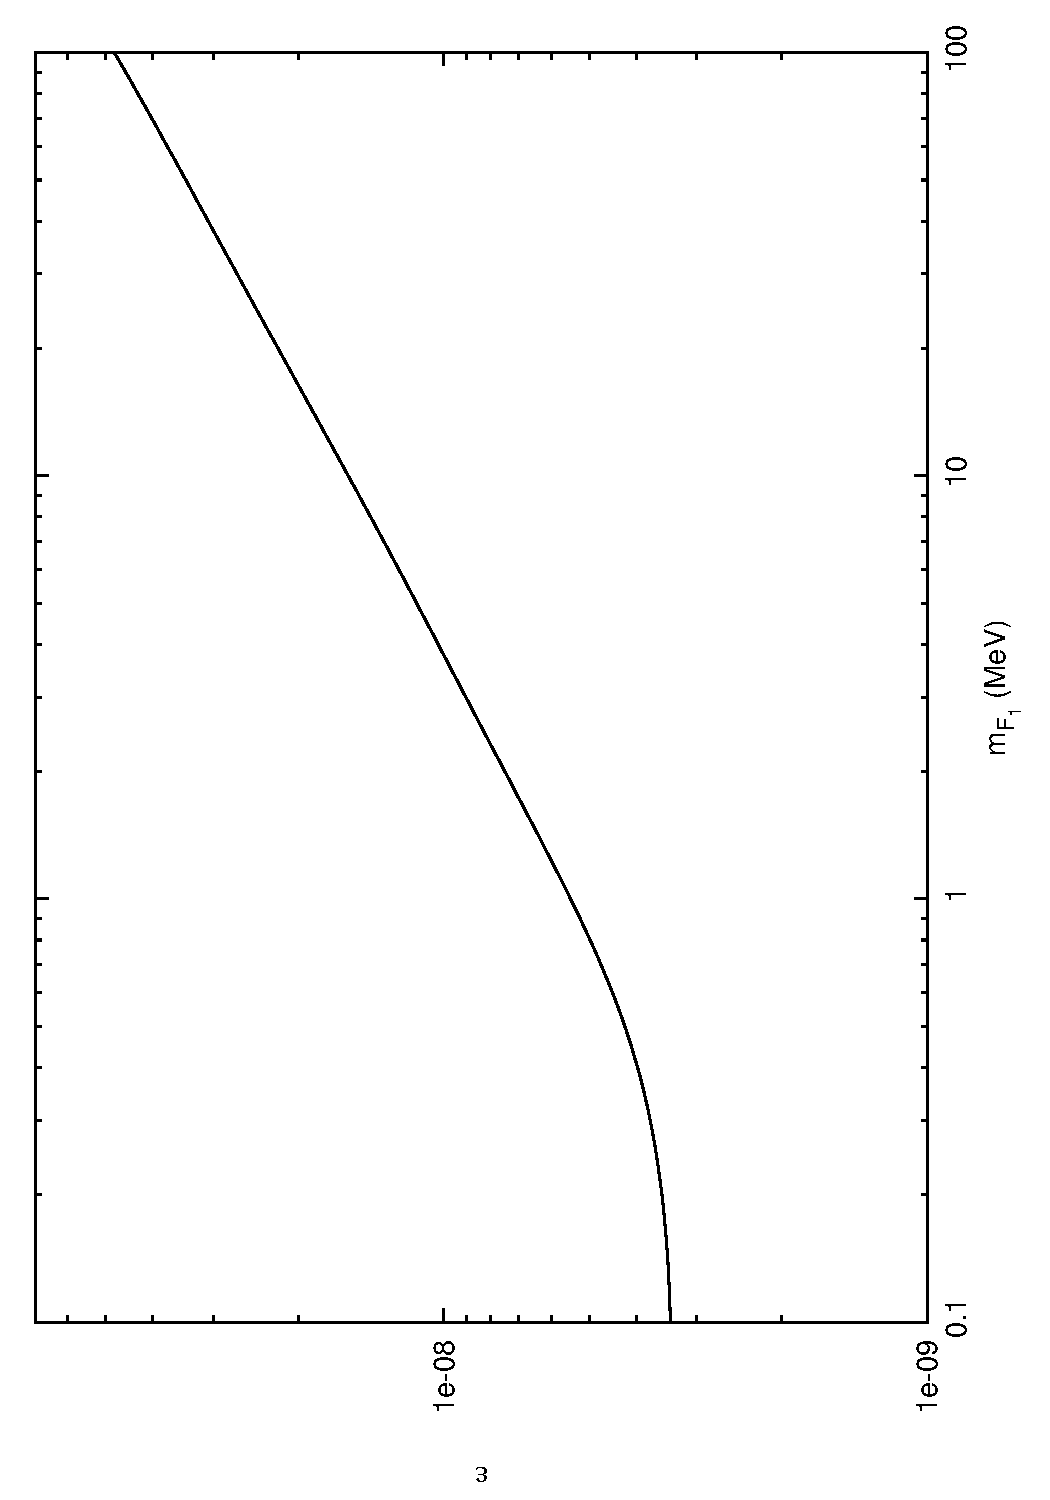
\includegraphics[width=.35\textwidth , angle=270]{fig9.eps}
%\vskip -0.4 cm
\caption{Difference between $\delta u(r)$ and $\delta u_{\text{th}}(r)$, to be compared with dashed line at $\Delta \delta u = 0$. CZB located at $r/R_{\odot} \simeq 0.73$.}
\label{fig7}
\end{figure}

Including helioseismological uncertainties yields the results shown in Figure \ref{fig7}, where we plot the difference $\Delta \delta u(r) \equiv \delta u(r) - \delta u_{\text{th}}(r)$. Being statistically independent, we add helioseismology uncertainties in quadrature with those propagated from uncertainties in the vSZ16 abundances. With helioseismological uncertainties correctly taken into account, we visually see that the agreement between $\delta u(r)$ and $\delta u_{\text{th}}(r)$ is very good. We construct a figure which puts the degree of compatibility on a more quantitative footing by averaging the quantity $\chi (r) \equiv \Delta \delta u(r)/\sigma (r)$ over the solar interior, $\sigma(r)$ denoting the 1$\sigma$ uncertainty on $\Delta \delta u(r)$ (blue band in Figure \ref{fig7}). We find that, adopting this measure, $\delta u(r)$ and $\delta u_{\text{th}}(r)$ are compatible within $\sim 1.4 \sigma$ [$\sim 0.6 \sigma$] when adopting statistical [conservative] uncertainties. In particular, at the CZB (where disagreement between previous models and helioseismology was most severe), the discrepancy is reduced to as little as $\sim 0.35 \sigma$ [$\sim 0.1 \sigma$] when using the statistical [conservative] approach. Above the CZB, the disagreement between model and helioseismology essentially disappears because the temperature gradient becomes adiabatic (consequently breaking hydrostatic equilibrium and causing convection to set in), and $u(r)$ depends no longer on the composition of the Sun. \newline \indent
%
Next, we compute the response of the surface He abundance using Eq.(\ref{kernel}). For $Y_s$, the SSM prediction is $\overline{Y_s} = 0.2356$ ($\pm 0.0035$ from modeling uncertainty), whereas the helioseismology value is $Y_s = 0.2485 \pm 0.0034$ (see e.g. \cite{psq2long}). Thus the (absolute) variation required to restore agreement is $\Delta Y_{s,\text{th}} \simeq 0.0129 \pm 0.0049$. Using Eq.(\ref{kernel}), the kernel $K_Y(r)$ shown in Figure \ref{fig3} and the opacity profile $\delta \kappa (r)$ shown in Figure \ref{fig2}, we find $\Delta Y_s \simeq 0.04 \pm 0.02$. Although the central value is in slight tension with that of $\Delta Y_{s,\text{th}}$, the involved errors are quite large and taking them into account the two are consistent within $\sim 1.3\sigma$. \newline \indent
%
Finally, we repeat the same analysis for the CZB. The SSM prediction $\overline{R_b}/R_{\odot} \simeq 0.722$ ($\pm 0.004$ from modeling uncertainty) is in tension with the helioseismology value of $R_b/R_{\odot} = 0.713 \pm 0.001$, the required fractional variation to restore agreement being $\delta R_{b,\text{th}} \simeq -0.012 \pm 0.005$. For the vSZ16 abundances we find $\delta R_b \simeq -0.008 \pm 0.004$, which is consistent with $\delta R_{b,\text{th}}$ within $\sim 0.6\sigma$. Our main results are summarized in Table \ref{tab2}. %\footnote{The shapes of $\delta \kappa (r)$ and $\delta u(r)$ are driven in a notable way by the changes in Si and S abundances, which are the largest ones within the catalogue. We explored the consequences of hypothetically neglecting $\delta Z_{\text{Si}}$ and $\delta Z_{\text{S}}$. This reduces the overall scale of $\delta \kappa (r)$ by $\sim 15$-$20\%$. For $\delta u(r)$, because of the size of the helioseismological uncertainties, the agreement with $\delta u_{\text{th}}(r)$ is basically unchanged. For $Y_s$ the agreement improves significantly. This occurs because the kernel $K_Y(r)$ is positive defined, making $\Delta Y_s$ sensitive to the overall scale of $\delta \kappa (r)$. We previously found the central value of $\Delta Y_s$ to be in slight tension with that of $\Delta Y_{s,\text{th}}$ because too large (albeit compatible at $1.3 \sigma$). Lowering the overall scale of $\delta \kappa (r)$ thus ameliorates the agreement, estimated at $\sim 0.4\sigma$. For $R_b$ the overall agreement is instead slightly degraded (from $\sim 0.7\sigma$ to $\sim 1.6\sigma$). The qualitative conclusion is that, once uncertainties are taken into account, the \textit{overall} agreement of the vSZ16 abundances with helioseismology is essentially unchanged whether or not the substantial changes of Si and S are accounted for.}.
\begin{table}[!h]
%\vskip -0.4 cm
\caption{Main results: response of helioseismological observables to change in abundance from AGSS09 \cite{agss09} to vSZ16 \cite{z16}, and compatibility with required variation.}
\label{tab2}
\begin{tabular}{c c c}
\hline\hline \vspace{-4mm}\\
 \ \ \ Observable \ \ \ & \ \ \ Variation \ \ \ & \ \ \ Compatibility \ \ \ \\      
\hline
 \ \ \ $Y_s$ \ \ \ & \ \ \ $0.04 \pm 0.02$ \ \ \ & \ \ \ $\sim 1.3\sigma$ \ \ \ \\
 \ \ \ $R_b$ \ \ \ & \ \ \ $-0.008 \pm 0.004$ \ \ \ & \ \ \ $\sim 0.6\sigma$ \ \ \ \\
 \ \ \ $\delta u(r)$ \ \ \ & \ \ \  \ \ \ & \ \ \ $\sim 1.4\sigma$\footnote{$\sim 0.6\sigma$ when using conservative helioseismological errors.} \ \ \ \\
\hline
\end{tabular}
\end{table}

\textbf{\textit{Discussion.\/}}\---We have reassessed the solar abundance problem in the light of new \textit{in situ}-determined metal abundances, finding that these restore the  agreement between models and helioseismology. The value of the metallicity determined is significantly higher than the findings of other groups based on photospheric spectroscopy. Moreover, since \textit{in situ} determinations actually provide a lower bound to the true value of the metallicity (due to possible residual fractionation), this suggests that previous determinations considerably underestimated the metallicity of our Sun. Individual element abundances change significantly with respect to previous findings as shown in Table \ref{tab1} (e.g. Si and S increase by $\gtrsim 100\%$). Using these new measurements of solar composition, we studied the response of helioseismological observables and present our main findings in Table \ref{tab2}, which shows that the disagreement between previous models and helioseismology is considerably alleviated. \newline \indent
%
It is beyond the scope of this analysis to address the specific problems of the spectroscopic methodology, which has determined a smaller metallicity and is inconsistent with helioseismology. There are nonetheless a number of these shortcomings which are being addressed in improved modern photospheric spectroscopy models currently being developed (e.g. \cite{caffau}): these include number of required opacity bins used and weight assigned to various lines, and that radiative transfer calculations most likely do not adequately estimate the impact of blending lines. \newline \indent
%
Recently proposed solutions to the problem based on exotic energy transport by captured DM are also severely disfavored. While this type of non-local energy transport can mildly ameliorate the discrepancy for $u(r)$ and $R_b$, this occurs at the expense of worsening the disagreement with $Y_s$ (which decreases as a result of core cooling, to which the Sun responds increasing its Hydrogen fraction) and lowering the neutrino fluxes beyond what is allowed by current measurements (e.g. \cite{vogel}). These and other issues will be discussed in more detail in a forthcoming work \cite{fssv}. \newline \indent
%
An independent observational constraint for these abundances resides in upcoming measurements of the CNO neutrino fluxes by SNO$^+$ \cite{sno}, which can lift the basic degeneracy between intrinsic and composition opacity variation \cite{villante1,villante2}. If the vSZ16 abundances are correct, such fluxes should be $\simeq$30-50$\%$ greater than reference predictions. These enhanced values are allowed by the existing rough upper limits from Borexino \cite{borexinophase1}. Similarly, we estimate a milder $\approx$10\% increase in the $^7$Be and $^8$B neutrino fluxes. This can mitigate the slight disagreement between AGSS09 abundances and measurements of these fluxes from Borexino \cite{be7,b8}, with the former predicting fluxes which are $\simeq$10\% lower than observed (see e.g. Table 2 in \cite{villante3}). \newline \indent
%
The possibility of confirming or disfavoring the revised abundances presented here is well within reach. Should our picture be confirmed, we will truly be able to claim that the solar abundance problem has been solved. \newline \newline \indent
%
KF and SV are supported by the Vetenskapsr\r{a}det (Swedish Research Council). THZ is partially supported by NASA NNX13AH66G. SV thanks the Michigan Center for Theoretical Physics for hospitality while this work was conducted. THZ acknowledges the International Space Science Institute in Bern, where much of the analysis relevant to this work has been performed. SV thanks Subir Sarkar, Ian Shoemaker, and especially Mads Frandsen for many fruitful discussions on the subject of the solar abundance problem, as well as Pat Scott and Francesco Villante for patiently answering many questions on the subject.

\bibliography{160305960}

\end{document}
